\subsection{Style extraction and handwriting reproduction}
\label{sec:des-reproduction}
The reproduction stage extracts single character, or glyphs from labelled handwriting, stores each writer's shape and spacing measurements, and then synthesizes them into new text.

\subsubsection{Choice of reproduction representation}
A glyph profile reuses the few labelled pages available for each author in the personal or IAM datasets. Haines et al. used approximately four A4 pages in their glyph-based experiments~\cite[p.~4]{haines2016}. The new sentences can be synthesized and created without the need for a heavy weight classifier trained on large amounts of data for reproduction, and is then mapped to the gantry.

The photographs contain no measured pen order, speed or pressure, unlike the trajectories required by recurrent synthesis~\cite[p.~18]{graves2013}, because the system used in this project was an offline system, performing computer vision on static images. Text synthesis that is based on image generatoration can work real time with very few existing style references as data, but the issue is an entire model still needs to be trained on much data, and requires a significant amount of computation to train the model well, for example on IAM-based synthesized image generator used 339 writers and four RTX 3090 GPUs~\cite[p.~9]{dai2024}. The chosen glyph approach fits the available data and compute, but has an expected weakness of performing glyph extraction on heavily connected authors. Various methods were implemented alongside the glyph extraction and synthesis, to improve the quality of reproduced writing.

\subsubsection{Character alignment and glyph extraction}
\label{sec:des-alignment}
A source line has a known transcript but no labels on where exactly each character is positioned. The existing trained text classifier supplies frame probabilities, and uses CTC forced alignment to select the highest-scoring path consistent with that ideal label or transcript. It uses the CTC transition rules, replacing path summation with maximisation~\cite[pp.~4--5]{graves2006}.
\begin{equation}
V(t,s)=\log p_t(\ell'_s)+\max_{r\inP(s)}V(t-1,r).
\label{eq:des-viterbi}
\end{equation}

where $\ell'$ is the text label interleaved with blanks and $ P(s)$ is the allowed predecessor set for state $s$. Backtracking gives each character's frame interval. A frame edge $t$ maps about to the source position $(640t/T)/a$, using the inverse canvas scale $a$. Multiple acceptable boundaries can still give the correct transcript.

The horizontal ink profile guesses the main box of the text. Its first and last rows above 45\% of the maximum calculate the band top and baseline $b$, with difference $h_x$ giving estimated x-height, and bands below three pixels are not used. Initial character cuts are refined towards thin connectors or blank columns using the project-specific cost
\begin{equation}
C_x=\frac{ p_x}{q_{0.60}( p_j: p_j>0)}
+1.15\operatorname{clip}\left(\frac{b-y_{\mathrm{top}}(x)}{h_x},0,3\right).
\label{eq:des-cutcost}
\end{equation}

where $p_x$ is smoothened column ink, the bottom of the equation is its positive-count 60th percentile, and $y_{\rm top}(x)$ is the highest ink row. The height term prefers lower connectors that are closer to the baseline. A true blank column has no cost. Cuts remain ordered, with minimum cell width being $\max(1,0.08h_x)$, so neighbouring boundaries can't collapse onto the same gap.

Figure~\ref{fig:des-alignment} follows the archived first Owen line because its crop and transcript can be traced through recognition and extraction. It shows the initial frame locations, refined cuts and resulting glyphs. The worked path and cut-cost substitutions are in Appendix~\ref{app:worked-design-calculations}.
\begin{figure}[H]\centering
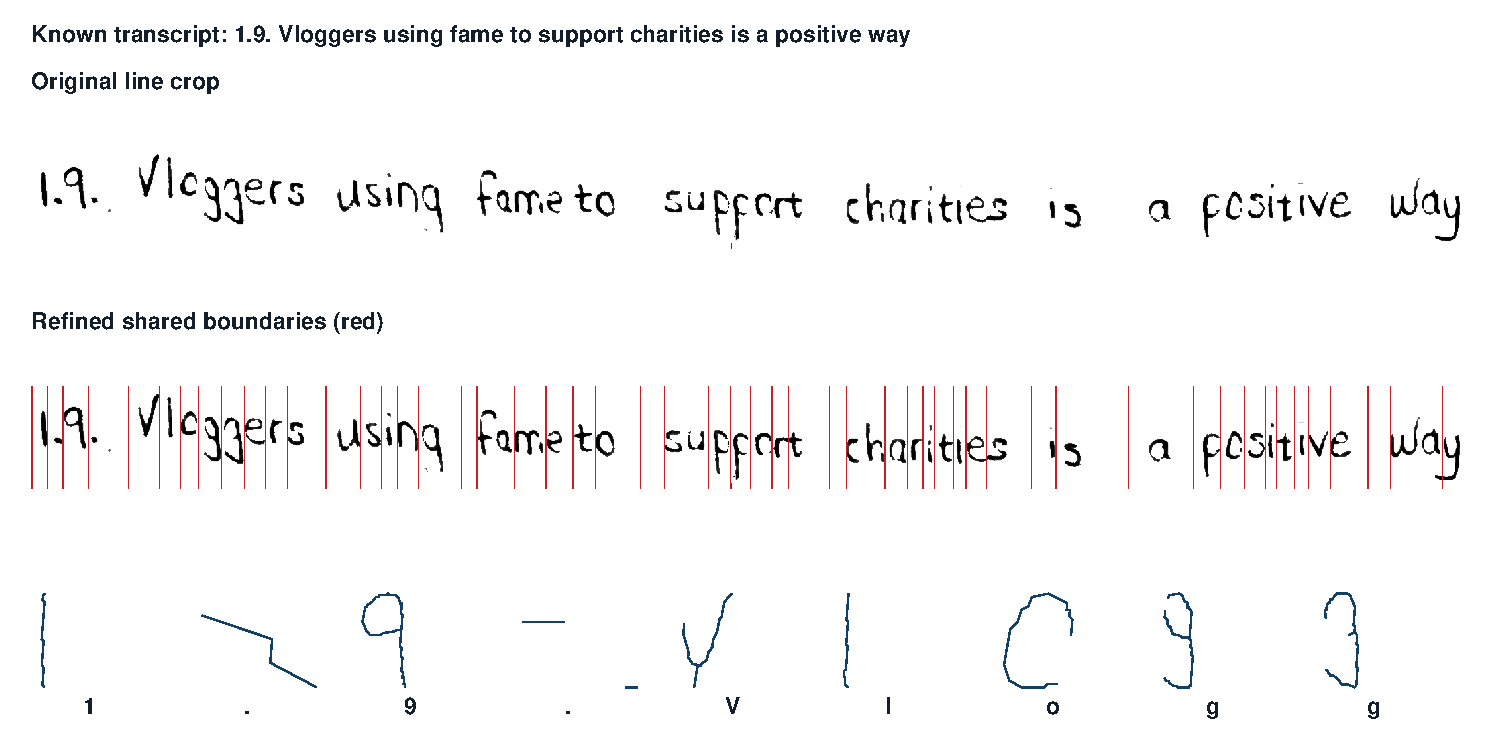
\includegraphics[width=0.96\linewidth]{Figures/design-glyph-alignment.pdf}
\caption{Character alignment and refined glyph cuts.}
\label{fig:des-alignment}
\end{figure}

\subsubsection{Skeleton tracing and pen path construction}
The process of thinning is used to convert an ink area into a one-pixel centreline, effectively reducing the thickness of any ink feature to one pixel width~\cite[p.~237]{zhang1984}. The complete line is thinned first before its cut into cells, to avoid an artificial thinning boundary generated at every letter. A graph tracer is used to divide paths at intersections, and eliminates short text artifacts and rejoins compatible ends that are below a $75^\circ$ continuation angle. The Douglas-Peucker simplification removes unnecessary vertices within a bounded deviation~\cite{douglas1973}. It works by drawing anchor lines betweem two ends of a line of text to create, and then finds the point of the text further away from the anchor. If the point is further than a limit value, the point is kept and made to be a new vertex. The Douglas-Peucker algorithm is mentioned in the literature review.

Dots that are on their own are recovered as short paths, and eligible detached crossbars (like for a 't' shape) are assigned to their letter rather than split across cells or counted as cursive joins between two letters. The resulting points are stored relative to left cut $x_L$, baseline $b$, x-height $h_x$ and slant $\phi$, using a shear transform~\cite{vinciarelli2001}.
\begin{equation}
v=\frac{b-y}{h_x},\qquad
u_0=\frac{x-x_L}{h_x}-v\tan\phi,\qquad u=u_0-\delta.
\label{eq:des-glyphcoords}
\end{equation}

The vertical coordinate increases upwards. The trim shift $\delta$ is removed from the stored horizontal path and kept as the lead-in spacing. Slant is removed for storage as a 'author feature' and is added again at placement. This separates the letter shape from its source size and cell spacing.

Figure~\ref{fig:vt-tracing} shows the Owen fragment before and after thinning and tracing. Across its full line, simplification reduces 3738 vertices to 974 at 0.6 source-pixel tolerance. The graph gives geometric paths, while the writer's original stroke order remains unknown. The coordinate substitution is retained in Appendix~\ref{app:worked-design-calculations}.
\begin{figure}[H]\centering
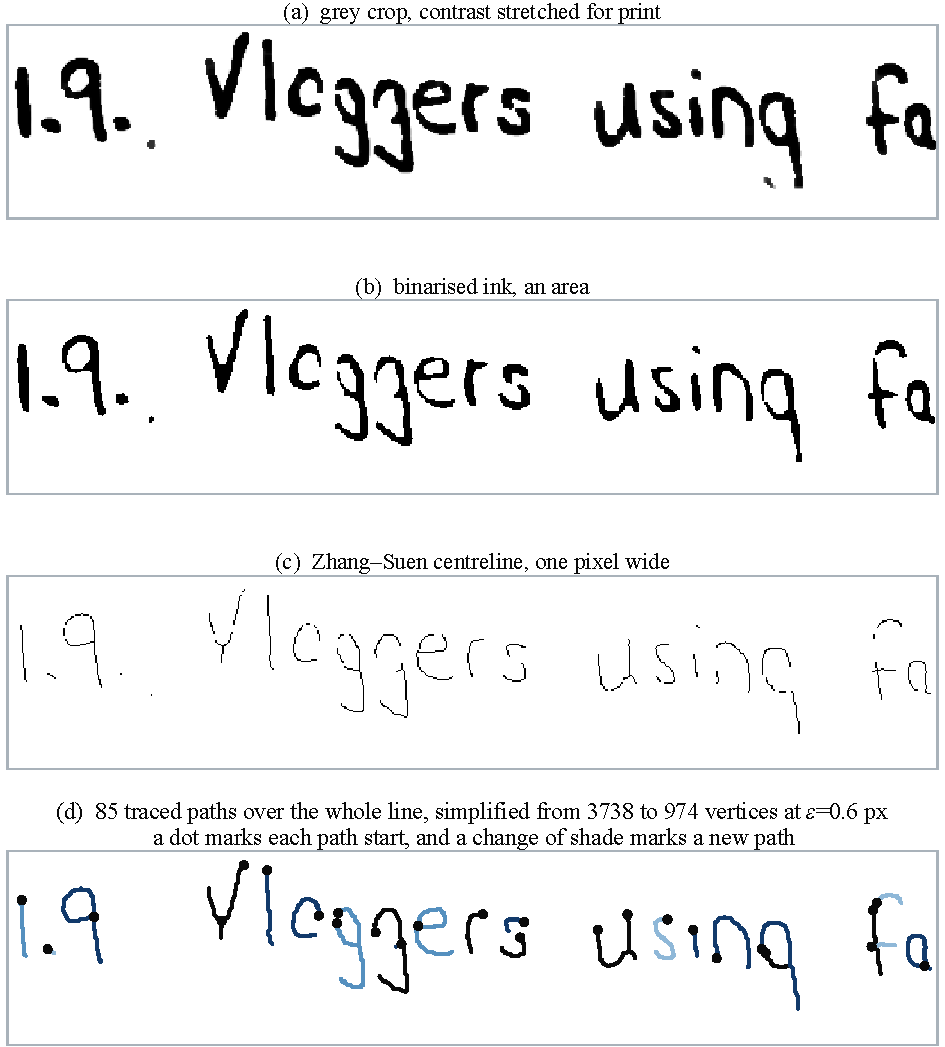
\includegraphics[width=0.96\linewidth]{Figures/VisualTests/T41_skeleton_trace_simplify.pdf}
\caption{Ink, skeleton and simplified pen paths.}
\label{fig:vt-tracing}
\end{figure}

\subsubsection{Glyph selection and library quality}
Alignment can place a cut inside a letter even when the text is correct, making the letter unusable, and is then an unreliable glyph. The profile therefore filters out and removes unreliable lines and glyphs using width, height, stroke count, path length and allocated character advance. This is why it is beneficial to have more lines and pages of training data to extract glyphs from, as it presents a higher chance of producing a decent looking glyph. Ordinary widths are limited to 2.1 x-heights and wide letters to 2.9. Distributions that are specific to certain characters provide further checks without forcing every letter to the same size.

A normalised $12\times12$ occupancy descriptor compares shape. A pooled character reference identifies cuts that are done incorrectly, while pairwise distances within a writer's pool identify a representative real variant, called the medoid. A mediod is effectively the geometrical average of multiple extracted glyphs, to produce the 'average' glyph for a specific character. A separate denoised prototype combines compatible strokes. The ordinary pool holds up to twelve variants per character. Algorithm~\ref{alg:des-profile} shows where these checks are done when creating a new profile. The descriptor distance is $d(g,c)=1-v_g^Tr_c$ for unit-normalised glyph descriptor $v_g$ and class reference $r_c$. The medoid is used to minimise the differences betweem the glyph distances per class.
\begin{designalgorithm}
\caption{Labelled handwriting to a persistent writer profile}
\label{alg:des-profile}
\prequire{Labelled original lines $L$, trained reader and writer identifier.}
\begin{designpseudo}
\pstate{0}{$G = null$; $S= null$}
\pstate{0}{\textbf{for each} $(G,l)\in L$ \textbf{do}}
\pstate{1}{$A=\operatorname{ForcedAlign}(G,l)$; estimate baseline, x-height and slant}
\pstate{1}{\textbf{if} alignment or body band is unusable \textbf{then continue}}
\pstate{1}{Refine shared increasing cuts, thin full line, and trace skeleton paths}
\pstate{1}{Split paths at cuts, assign crossbars, recover untraced dots}
\pstate{1}{Normalise glyph coordinates, and record advance, lead and boundary crossings}
\pstate{1}{Append glyphs to $G$ and line measurements to $S$}
\pstate{0}{\textbf{end for}}
\pstate{0}{Cache raw extraction; reject low-confidence lines relative to this writer}
\pstate{0}{\textbf{for each} character's glyph pool $G_c$ \textbf{do}}
\pstate{1}{Apply size, height-class, path-length and cell-consistency gates}
\pstate{1}{Refine size range, and apply cross-writer prior and within-writer consensus}
\pstate{1}{Rank and smooth retained variants, and construct medoid and eligible prototype}
\pstate{0}{\textbf{end for}}
\pstate{0}{\textbf{return} persistent profile containing $G$ and robust summaries of $S$}
\end{designpseudo}
\end{designalgorithm}

Figure~\ref{fig:des-profile-example} compares the nine stored \texttt{a} variants for Owen, Dylan and Yeukita. The cloud shows their variation, the medoid is an actual example, and the prototype is a combined shape. The distance bars explain which variant is most typical within each writer. The exact descriptor and medoid calculations are retained in Appendix~\ref{app:worked-design-calculations}.
\begin{figure}[H]\centering
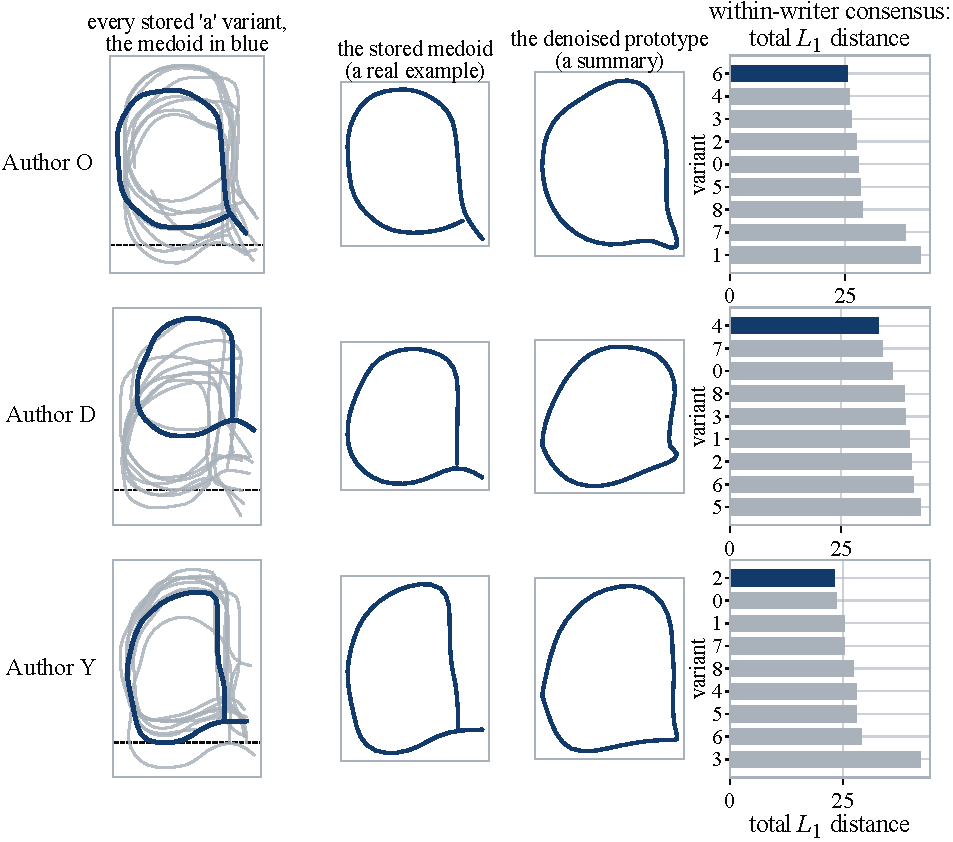
\includegraphics[width=0.98\linewidth]{Figures/VisualTests/T45_variant_pool_medoid.pdf}
\caption{Glyph variants and representatives for three writers.}
\label{fig:des-profile-example}
\end{figure}

Missing characters can use case-related shapes, similar forms or fallback glyphs, known as 'anchor glyphs'. When a character is missing, or is too incomplete to be used, the anchor glyph will be pulled instead (different cases exact for separate and cursive styles). They allow text generation to continue, but a fallback does not establish that the character was captured in that writer's style, but since certain author's features are still extracted and applied afterwards, the anchor glyph still gets certain author's style traits applied to it.

\subsubsection{Writer style measurement and storage}
\label{sec:des-profile}
A profile of each author's features is created per author, which stores slant, x-height, ascender and descender extent, character advance, word gap and percentage connectivity coefficient. Slant is estimated by finding the shear that concentrates ink into columns, and dimensions of the text are normalised by x-height to reduce the dependency on the resolution of the image taken.

Connectedness is the percentage amount of available adjacent non-space boundaries crossed by a traced centreline, which is a method motivated by contour-based writer features~\cite[p.~701]{bulacu2007}.
\begin{equation}
c=\frac{N_{\mathrm{cross}}}{\max(1,N_{\mathrm{adj}})}.
\label{eq:des-connectedness}
\end{equation}

\subsubsection{Text layout and connected handwriting synthesis}
\label{sec:des-layout}
The synthesiser selects glyph variants, applies the stored style and places words within the available line width. Character advance, which the effective width of characters based on author style, and word gap come from the profile. Words will move onto the next line when the remaining width is insufficient.

For stored point $(u,v)$ and lead $l$, physical x-height $h_x^{\rm mm}$ converts the glyph to millimetres. Slant shear $s$ and baseline drift $d$ modify the generated text about placement origin $(p_x,p_y)$.
\begin{equation}
x=p_x+h_x^{\mathrm{mm}}(l+u+sv),\qquad
y=p_y+h_x^{\mathrm{mm}}(v+d).
\label{eq:des-placement}
\end{equation}

Small linear shifts, rotations and scale changes provide some variation to the text that is created. Drift changes gradually with persistence 0.85 and is bounded to $\pm0.25$ x-heights, and 0.05 x-height clearance limits collisions. Variants that are better are sampled more often, with two variants with similar entry heights preferred for joining, since they would look more natural being next to one another.

The value of the automatic anchoring strength $\lambda$ depends on median stored prior distance $d$.
\begin{equation}
\lambda=\operatorname{clip}\left(\frac{d-0.24}{0.32-0.24},0,1\right).
\label{eq:des-anchor}
\end{equation}

Lower-distance attempts tend to keep more personal variants. Larger distances increase the dependence on an acceptable representative of the available glyphs, and then a generic form from the anchor set if needed. 

Joining uses the writer's measured connection fraction, but is suppressed below 0.45, due to the fact that connections could be detected incorrectly during forced alignment and boundary cutting, adding too many unnecessary connections for simple writing that is not cursive. Authors about the threshold tend to be somewhat heavy and connected cursive writers, so more connections is preferred. A join also requires a compatible source and gap no greater than 0.80 x-heights, to prevent long, unnatural looking line connections between distance characters. A shallow connector joins the body strokes without attaching to dots or crossbars. A rendered probe applies bounded slant and extent corrections before synthesis. The placement and anchoring examples are retained in Appendix~\ref{app:worked-design-calculations}.

\subsubsection{Candidate selection for legibility and writer identity}
\label{sec:des-selection}
The different selections of glyph choices can change the readability and writer identity. Each candidate is rendered at constant ink width and scored by the reader and stroke-normalised author classifier. Character score $A$ and requested-writer probability $P$ form joint score $J$.
\begin{equation}
A=\max\left(0,1-\frac{d_{\mathrm{edit}}(\widehat t,t)}{|t|}\right),\qquad
J=\begin{cases}2AP/(A+P),&A+P>0,\\0,&\text{otherwise}.\end{cases}
\label{eq:des-jointscore}
\end{equation}

The harmonic mean punishes a candidate weak in either score and will give priority to another attempt. The recorded Author O candidate has $A=18/19=0.95$ and $P=0.58$, giving $J=0.72$. Algorithm~\ref{alg:des-joint} gives the bounded search and repair sequence. A repair is retained only when the complete candidate score improves.
\begin{designalgorithm}
\caption{Joint candidate search and bounded legibility repair}
\label{alg:des-joint}
\prequire{Text, writer profile, reader, shape classifier, seed $s$ and trial budget $K$.}
\begin{designpseudo}
\pstate{0}{$J^*=-1$; $R=0$; determine anchoring strength}
\pstate{0}{\textbf{for} $k=0$ \textbf{to} $\max(1,K)-1$ \textbf{do}}
\pstate{1}{$T=\operatorname{SynthesizeText}(\text{text},\text{profile},s+977k)$}
\pstate{1}{$I=\operatorname{RenderUniformInk}(T)$; $(A,P,J)=\operatorname{Score}(I)$}
\pstate{1}{\textbf{if} $J>J^*$ \textbf{then} $(T^*,I^*,J^*)=(T,I,J)$}
\pstate{1}{\textbf{if} $J^*\geq0.99$ \textbf{then break}}
\pstate{0}{\textbf{end for}}
\pstate{0}{\textbf{for} at most three configured repair rounds \textbf{do}}
\pstate{1}{\textbf{if} $J^*\geq0.995$ \textbf{then break}}
\pstate{1}{$W=$ up to two weak aligned positions not already in $R$}
\pstate{1}{\textbf{if} $W=0$ \textbf{then break}}
\pstate{1}{$R'= R\cup W$; regenerate with stronger anchors at $R'$ and seed $s$}
\pstate{1}{Render and rescore the complete trial trajectory}
\pstate{1}{\textbf{if} $J>J^*$ \textbf{then} commit $R'$ and the new best trajectory}
\pstate{0}{\textbf{end for}}
\pstate{0}{\textbf{return} $T^*$ with selection and accepted-repair metadata}
\end{designpseudo}
\end{designalgorithm}

Figure~\ref{fig:des-candidates} compares the three recorded trials of ``Writing with style.'' using the same profile and settings. Candidate 1 is selected because its writer score is stronger while retaining the same character score as candidate 3. The full values are in Appendix~\ref{app:worked-design-calculations}.
\begin{figure}[H]\centering
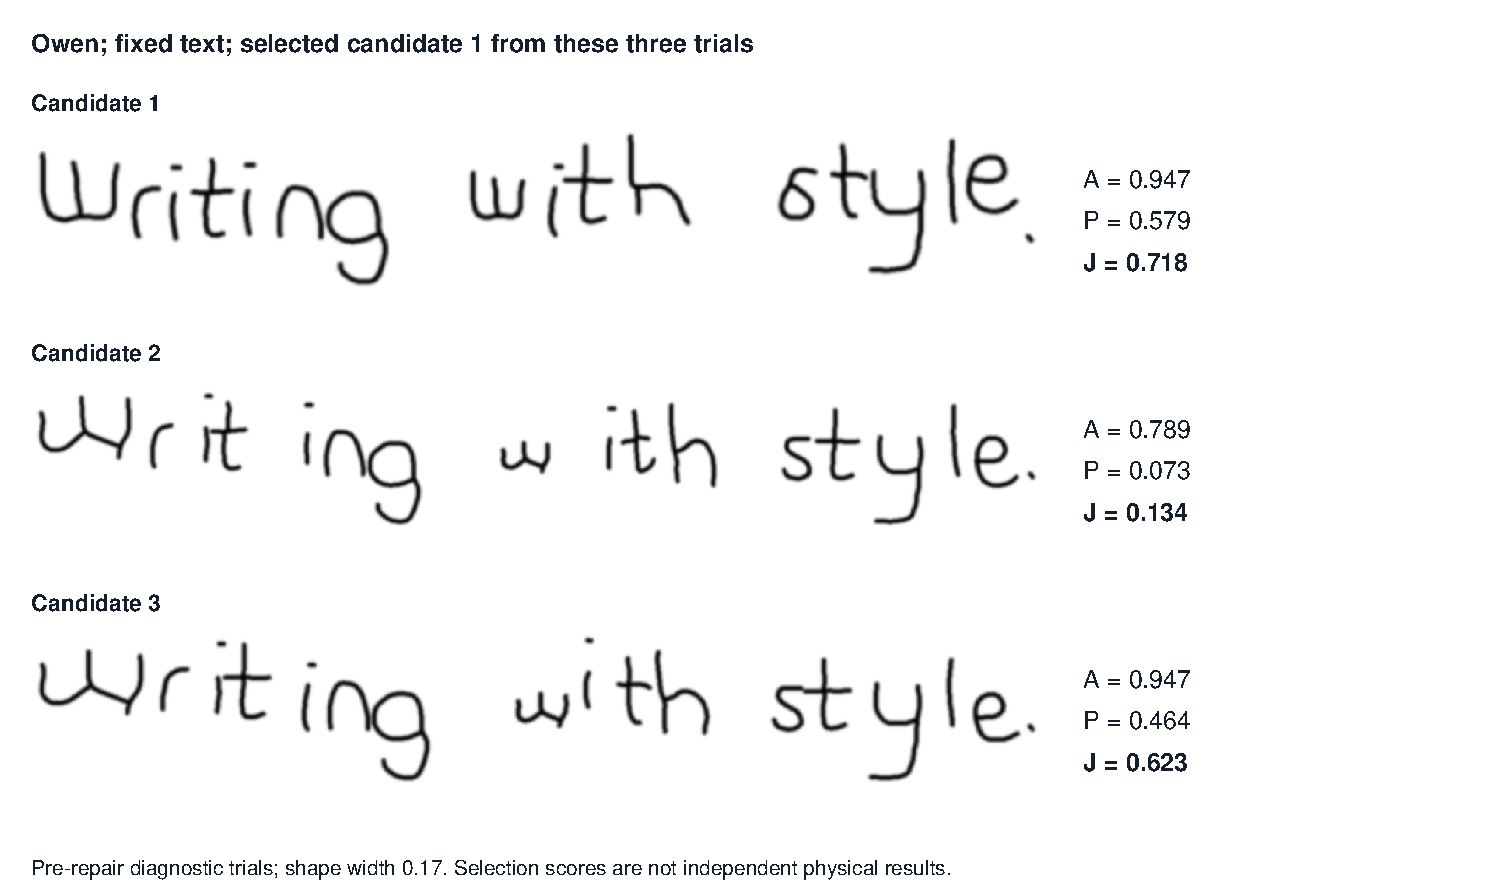
\includegraphics[width=0.95\linewidth]{Figures/design-candidate-selection.pdf}
\caption{Candidate paths and their selection scores.}
\label{fig:des-candidates}
\end{figure}

The scoring models only guide the choice of glyphs used, so their confidence does not independently prove physical style similarity. More trials also add inference time and cannot recover a missing source letterform, so there is a hard limit to the effect of running more trials, the system is always limited by the quality of the glyph.

\subsubsection{Machine coordinate mapping and G-code generation}
\label{sec:des-gcode}
The selected trajectory is fitted inside the calibrated workspace. The system contains a ruled placement option, where the user can select the line to begin the placement of the trajectory, while free placement retains its synthesised pitch. Character size and line spacing remain separate so that a tall descender need not change both.

Trajectory bounds $(x_0,y_0,x_1,y_1)$, origin $(o_x,o_y)$, margins $m_x,m_y$ and scale $a$ affect how the mapping is generated. Offset $d_y$ selects a later starting line and $\Delta_y$ adjusts line spacing.
\begin{equation}
x_m=o_x+m_x+a(x-x_0),\qquad
y_m=o_y-m_y-d_y-a(y_1-y)+\Delta_y.
\label{eq:des-machinecoords}
\end{equation}

Both stored and machine coordinates use upward-increasing $y$. Clamping is a final travel limit and can distort a letter. Robust extent fitting and margins should keep the generated text inside the bed before execution. Nearby path segments may be simplified and compatible strokes joined, using a default join distance of 0.6\,mm.

Figure~\ref{fig:des-gcode-excerpt} gives the opening commands of the generated Author O example. It selects millimetres, absolute coordinates, a movement where the pen is lifted, and the first drawing movements. The full point mapping and file interpretation are extended in Appendix~\ref{app:worked-design-calculations}.
\begin{figure}[H]
\begin{lstlisting}[style=designcode]
G21
G90
G0 F2400
G0 F2400 X15.000 Y240.557
M3
G4 P0.350
G1 F900
G1 X15.001 Y240.207
G1 X15.002 Y239.857
G1 X15.003 Y239.506
G1 X15.005 Y239.156
G1 X15.006 Y238.806
G1 X15.007 Y238.456
\end{lstlisting}
\caption{Opening commands of the Owen example.}
\label{fig:des-gcode-excerpt}
\end{figure}

Travel feed is restated after drawing because feed is modal. Waiting for the pen to reach its UP state adds 0.35\,s per transition to the switch-confirmed actuation. For drawing and travel distances $D_d,D_u$, feeds $F_d,F_u$ and $N_p$ alternating pen transitions, the nominal budget is
\begin{equation}
t_{\mathrm{nom}}=\frac{60D_d}{F_d}+\frac{60D_u}{F_u}
+\frac{N_p(t_{\mathrm{up}}+t_{\mathrm{down}})}{2}.
\label{eq:des-timebudget}
\end{equation}

The earlier traced file gives 32.82\,s, including 19.60\,s dwell. Figure~\ref{fig:vt-timeparts} shows a separate four-profile calculation for the same sentence. Waiting for the pen between state transitions makes up about 61 to 65\% of the total time. This identifies a motion-side improvement to test, while actual completion also includes synthesis, actuation and pulse-loop overhead.
\begin{figure}[H]\centering
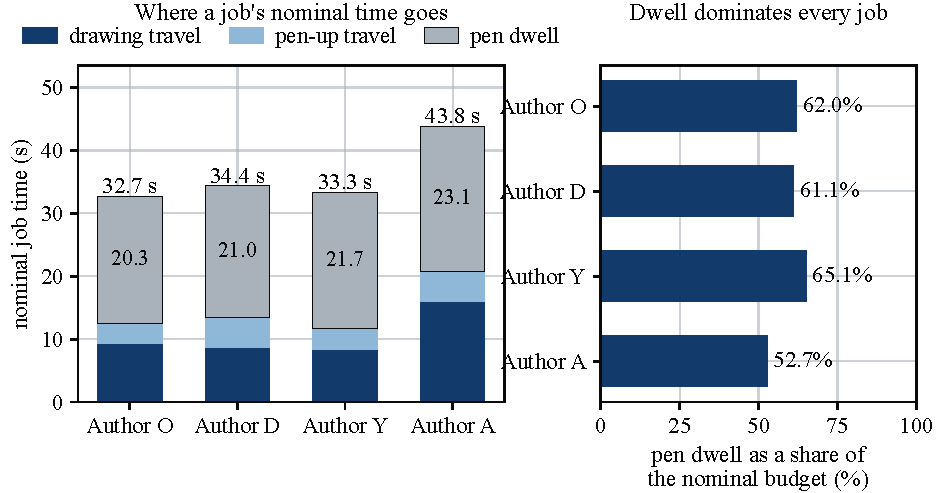
\includegraphics[width=0.96\linewidth]{Figures/VisualTests/T56_time_budget.pdf}
\caption{Drawing, travel and pen-dwell budgets.}
\label{fig:vt-timeparts}
\end{figure}

\subsubsection{Reproduction design limitations}
Most of the design limitations with the software part of text reproduction come from the engineering decision to use glyph-based text synthesis over a generative model. The reasons why a generative model was not used was discussed at the beginning of the section. The fundamental limitation with glyph extraction is the difficulty faced when attempting to perform forced alignment and single character glyph extraction on a heavily connected or cursive style. Through techniques like the glyph anchor usage when extracted glyphs fail, the connectedness coefficient, and reapplication of extracted author's features, allow some clean cursive variants to perform well. Heavy cursive is still a barrier and if more data and computational power was available, a generative model should be looked into to perform sentence generation.
\FloatBarrier
